\documentclass[a4paper, UKenglish, 11pt]{uiomaster}
\usepackage{lipsum}
\usepackage[subpreambles=true]{standalone}

% Explain EEG
% Explain how EEG sources can be modeled/simulated (include the first attempt done in 1949)
% Head models (New York Head Model)
% Maybe there should be an implementartion section ?

\begin{document}
\chapter{Results}
As mentioned in chapter 1, an important topic in EEG signal analysis is the inverse problem of going from measured EEG signals to localized equivalent current dipoles, so-called source localization. In this chapter we will be training and presenting two different(?) neural networks used to localize single dipole sources in the human cortex. Section ... and ... deal with training a simple feed forward neural network and presenting its results, while section ... will .

\section{The dataset}
The cortex matrix of the New York Head Model (NYHM) consists of 74382 points, which refer to the number of possible positions for localization of a dipole source. When training the FFNN we will be using a data set consisting of simulated EEG signals corresponding to dipol sources with randomly selected positions within the cortex matrix. The final data set consists of 10 000 rows, where each row corresponds to one sample, or let us say - one patient. Within the data set we have 231 columns, also referred to as features, representing the dipole measure at every EEG electrode. Thus, we are left with a design matrix with size 10 000 x 231.



% Maybe this does not belong here?
In order to train the network faster, one commonly split the data set into mini-batches, which is also done here. When splitting the data such a way, the weights of connection between neurons are updated after each propagation, making the network converge considerable faster.


% Scaling
% Every potential distribution presented to the network is first average referenced by subtracting the average of all potential values. Subsequently, the average referenced potentials are normalized by dividing them by the magnitude of the largest. The dipole location parameters are normalized to 1 with respect to the radius of the outer head boundary in the spherical head model (9.2 cm). In the case of a realistically shaped head model, the location parameters are normalized with respect to the radius of the best-fitting sphere for the scalp–air interface.

% As was pointed out in the previous section, the optimal dipole orientation (in the leastsquares sense) for a given location can be calculated in a straightforward manner. Therefore, we will use neural networks to estimate only the dipole location parameters.

\section{Simple example}

\begin{figure}[!htb]
    \centering
    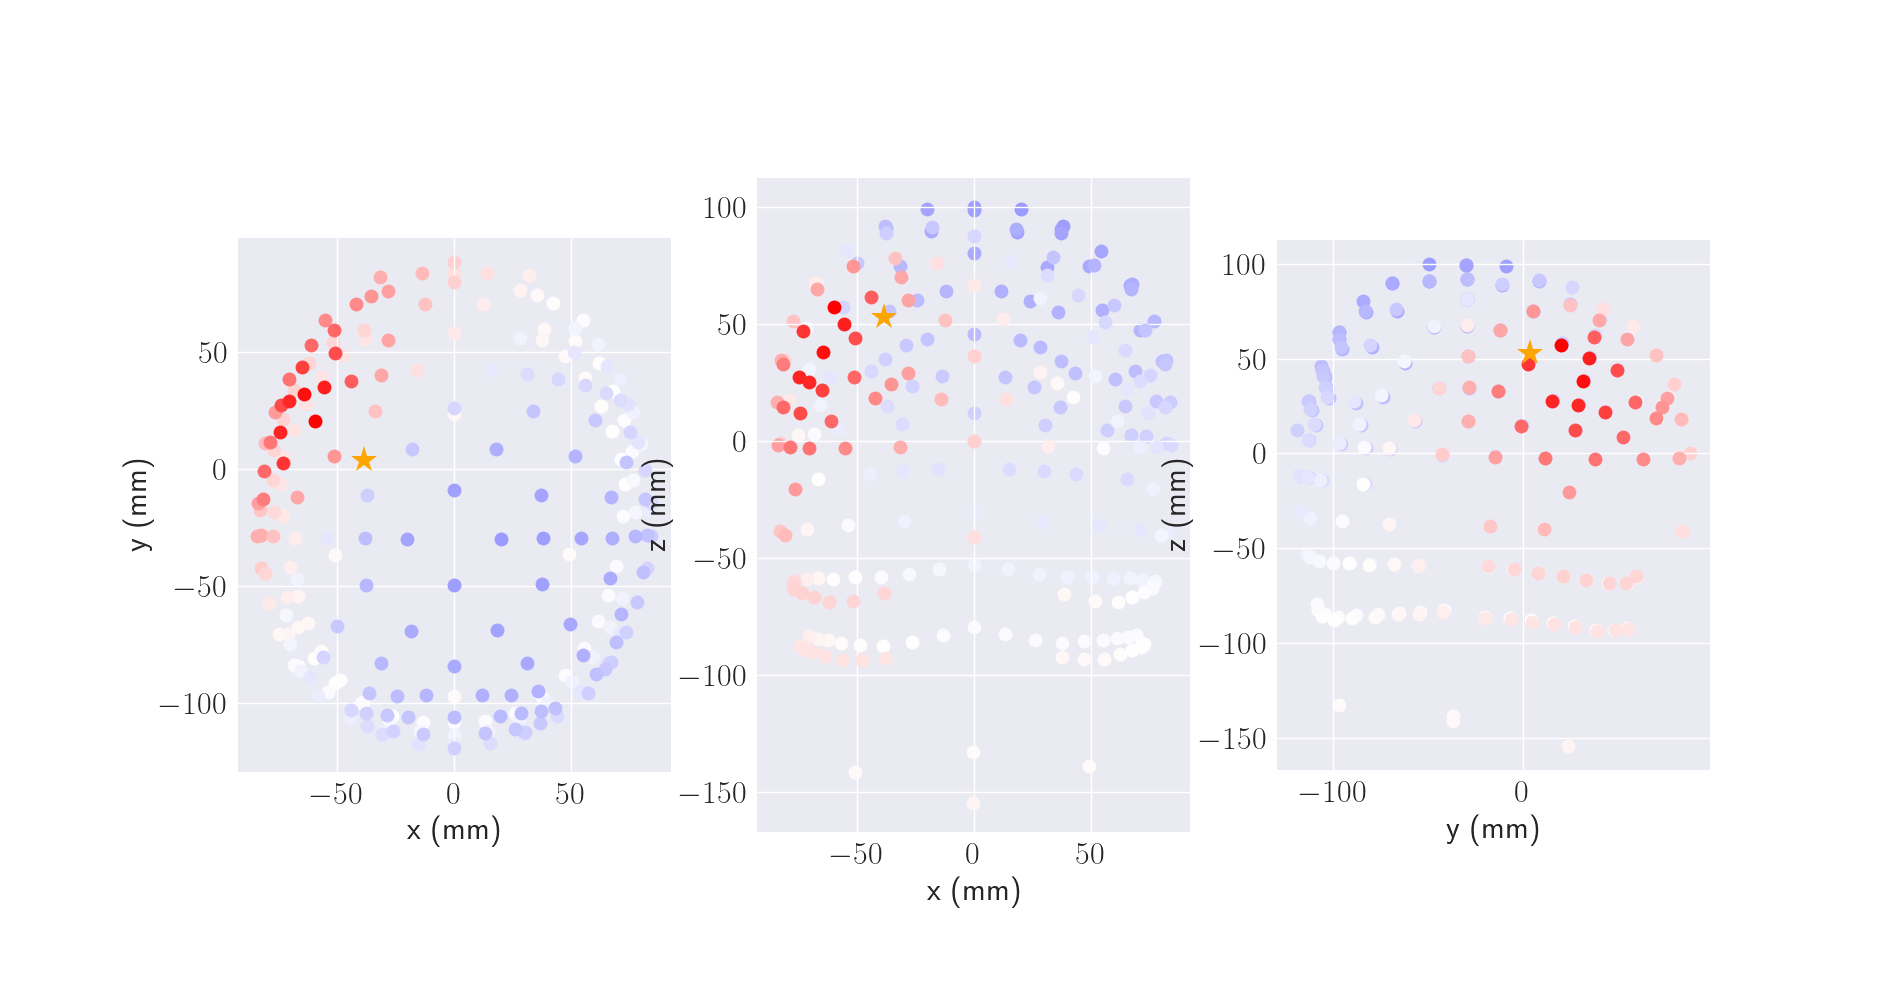
\includegraphics[width=\linewidth]{../Code/plots/finals/eeg_field_1_1.png}
    \caption{Example 1 dipole. }
    \label{fig:eeg_field_1_dipole_example}
\end{figure}

\begin{figure}[!htb]
    \centering
    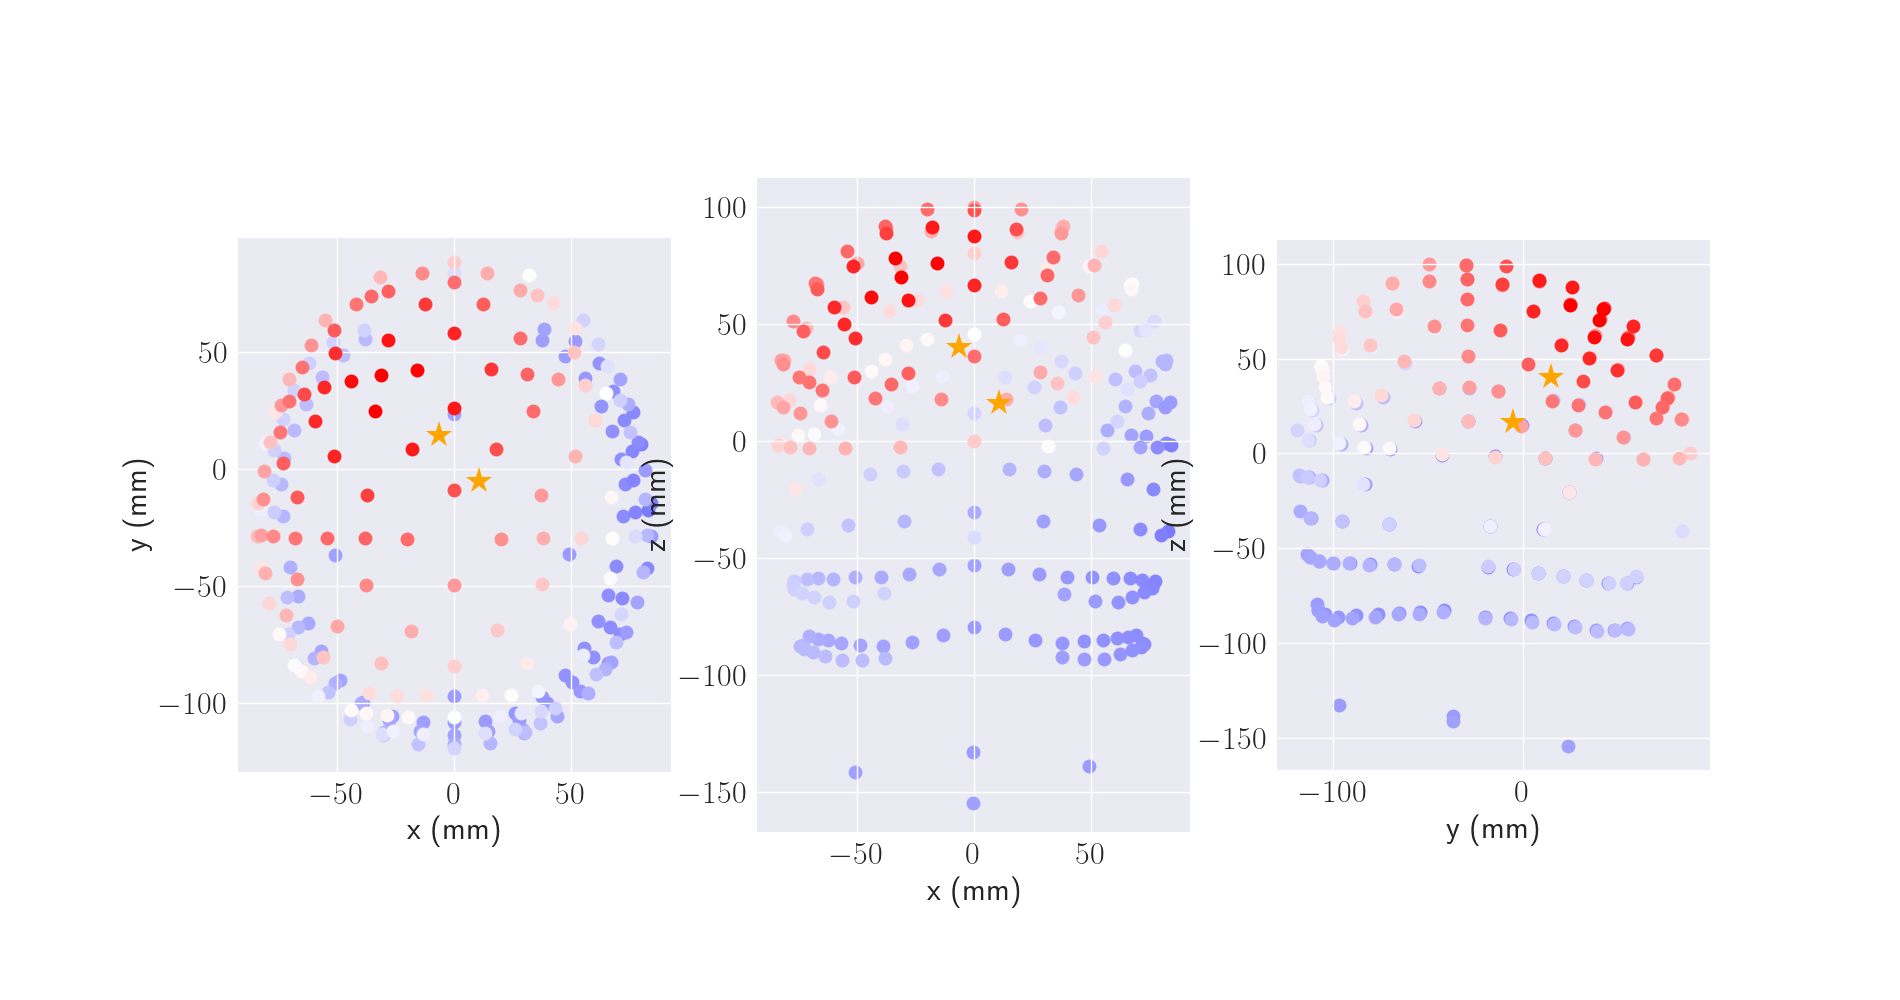
\includegraphics[width=\linewidth]{../Code/plots/finals/eeg_field_2_2.png}
    \caption{Example 2 dipoles. }
    \label{fig:eeg_field_2_dipole_example}
\end{figure}



\begin{figure}[!htb]
    \centering
    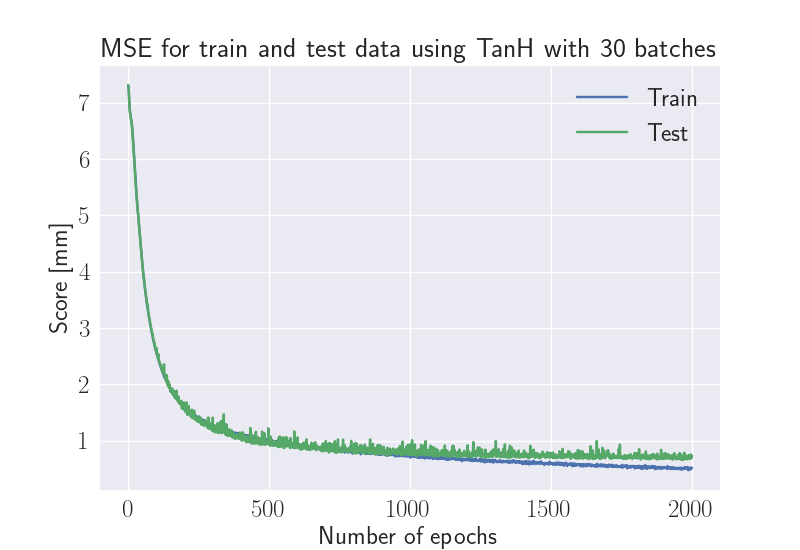
\includegraphics[width=\linewidth]{../Code/plots/finals/MSE_**multiple_dipoles_1_noise10_TanH_30_2000.png}
    \caption{The validation accuracy for simple Feed Forward Neural Network with 10 000 samples with tanh activation function. }
    \label{fig:single_dipole_accuracy}
\end{figure}

% \begin{figure}[!htb]
%     \centering
%     \includegraphics[width=\linewidth]{../Code/plots/NN/MSE_NN_noise_TanH_100_3000.png}
%     \caption{The validation accuracy for simple Feed Forward Neural Network with 10 000 samples with tanh activation function and 10$\%$ noise added to the data. }
%     \label{fig:single_dipole_accuracy}
% \end{figure}

\begin{figure}[!htb]
    \centering
    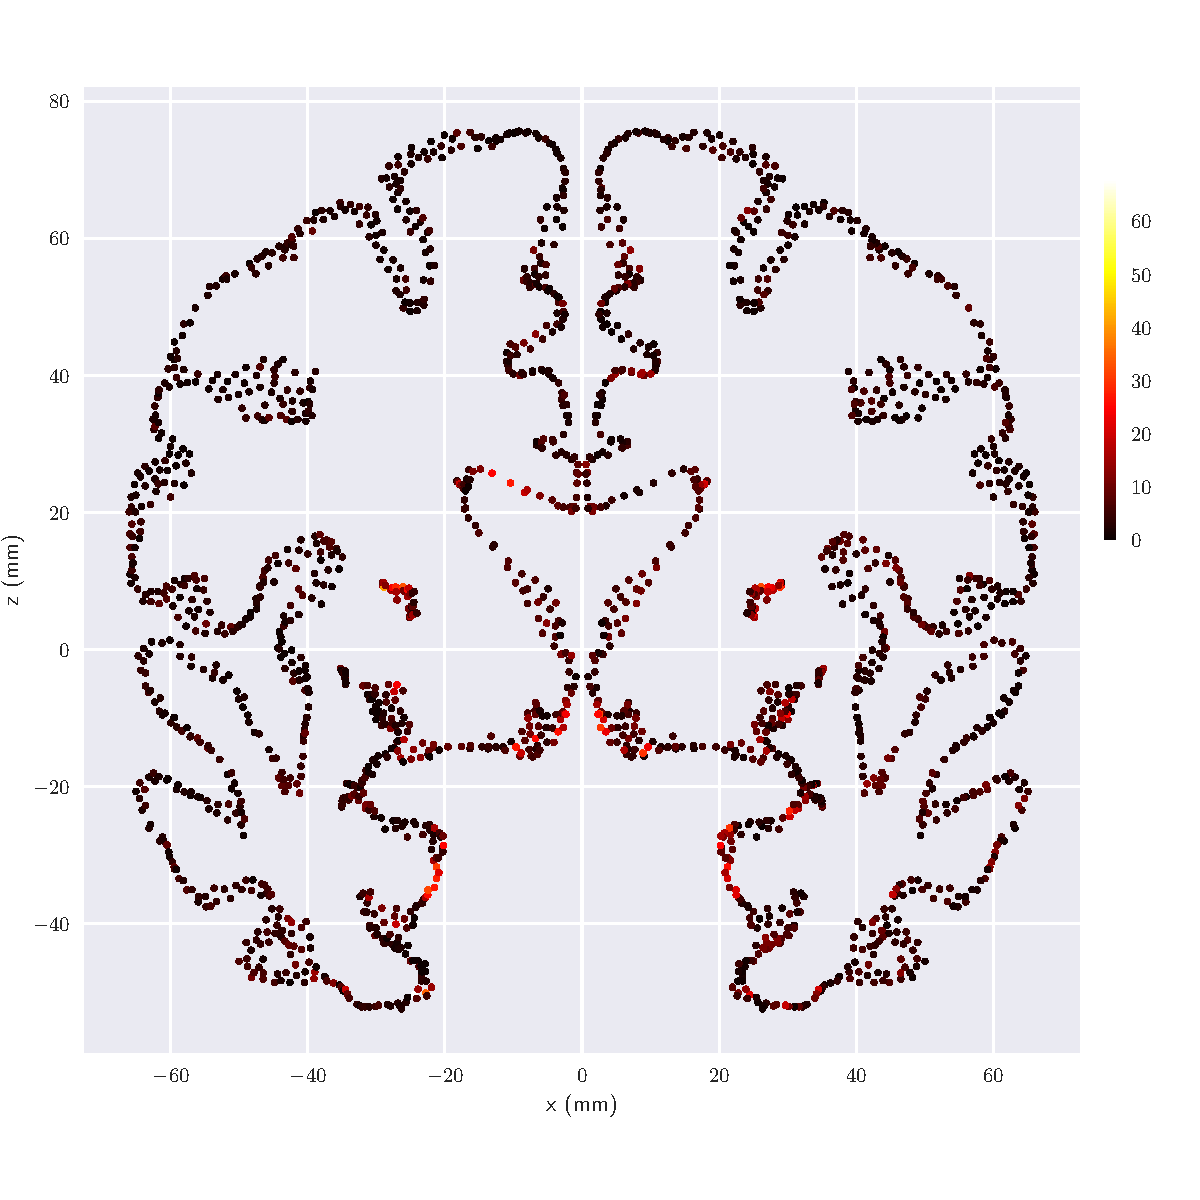
\includegraphics[width=\linewidth]{../Code/plots/finals/mse_y_plane.pdf}
    \caption{The mean squared error of the location accuracy (NN) at different dipole locations
    in the y cross section.}
    \label{fig:single_dipole_accuracy}
\end{figure}



\section{Convolution Neural Network Approach for localizing single dipole sources}

Some results for the prediction of location for single current dipoles.


\begin{figure}[!htb]
\centering
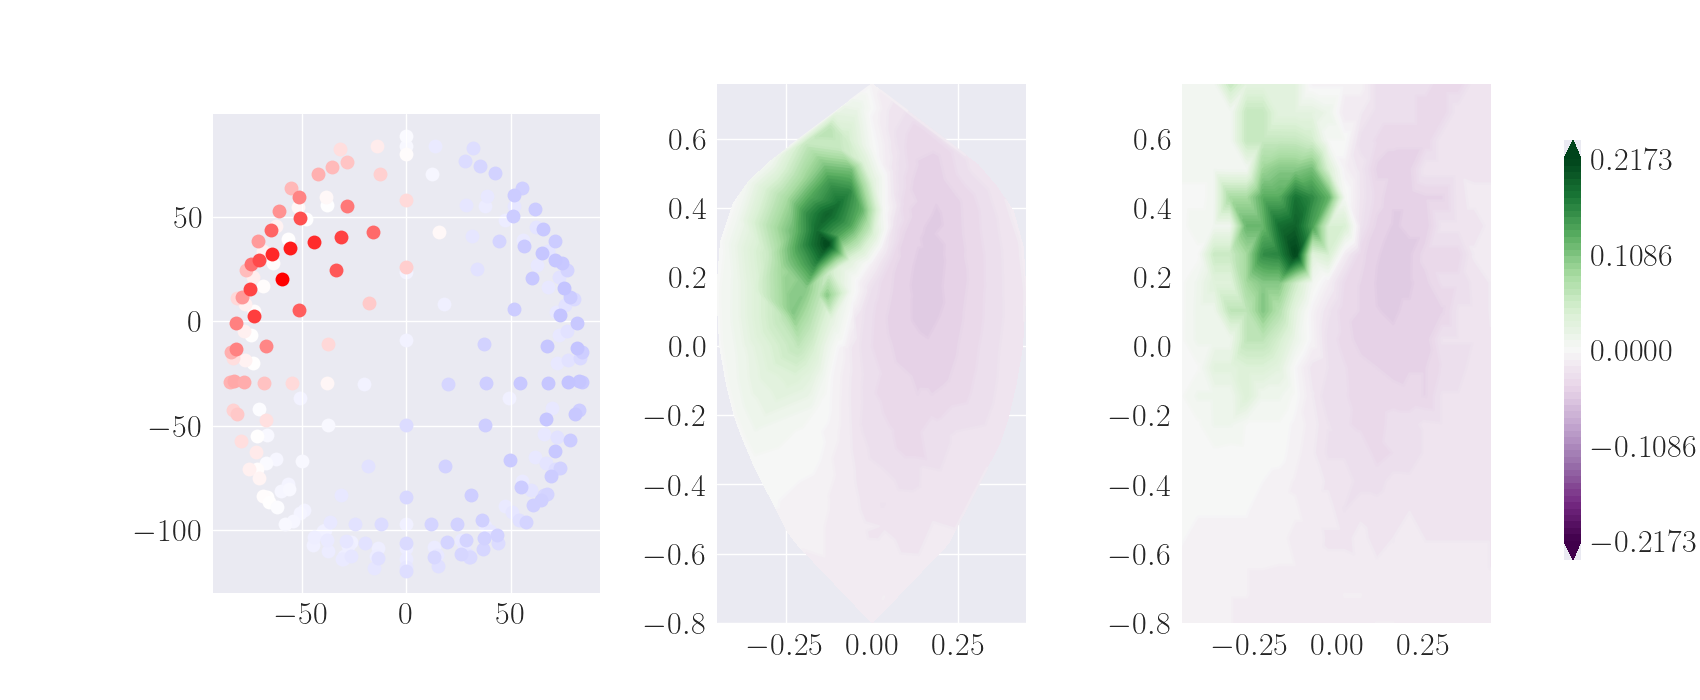
\includegraphics[width=\linewidth]{../Code/plots/finals/new_eeg_dipole_pos_0.png}
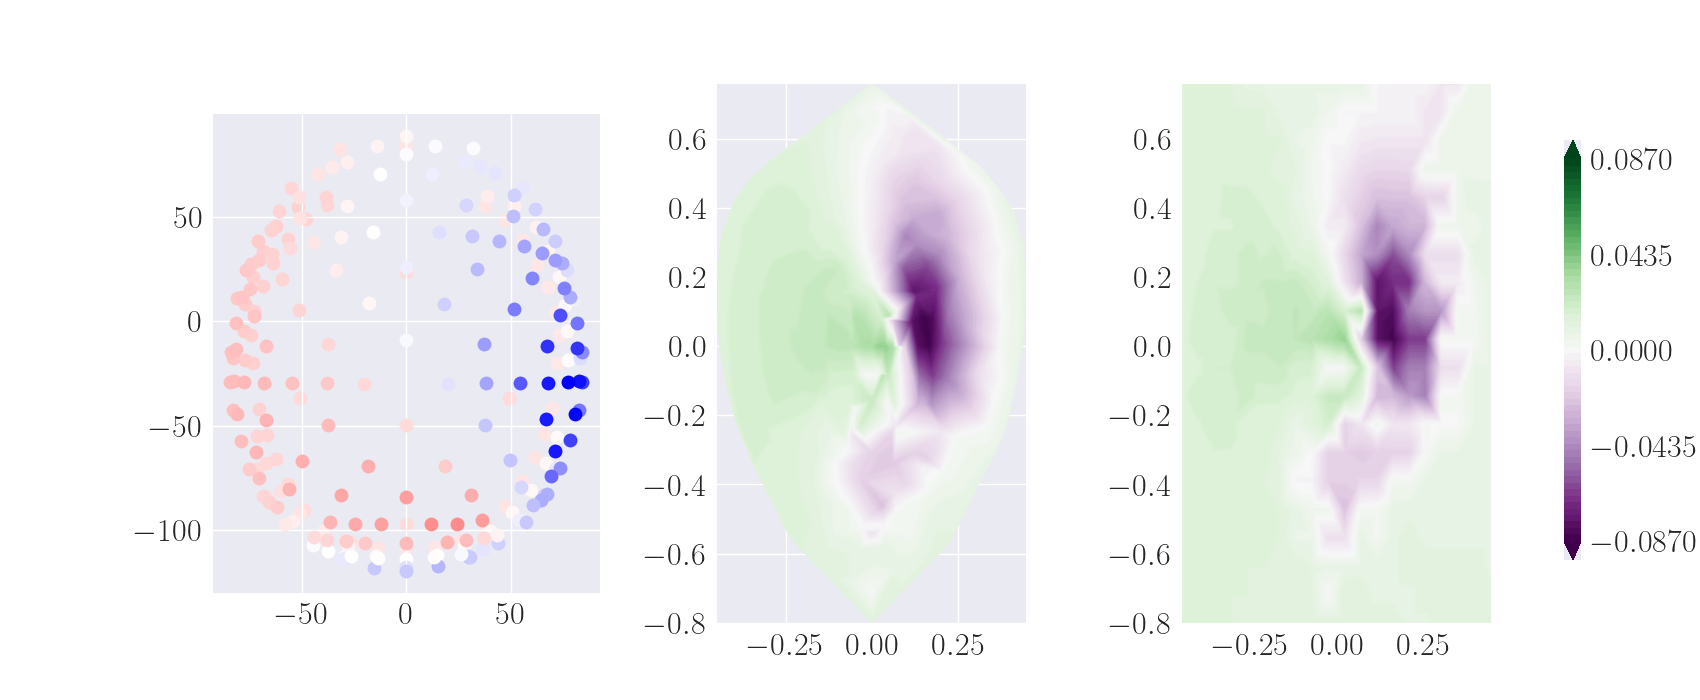
\includegraphics[width=\linewidth]{../Code/plots/finals/new_eeg_dipole_pos_4.png}
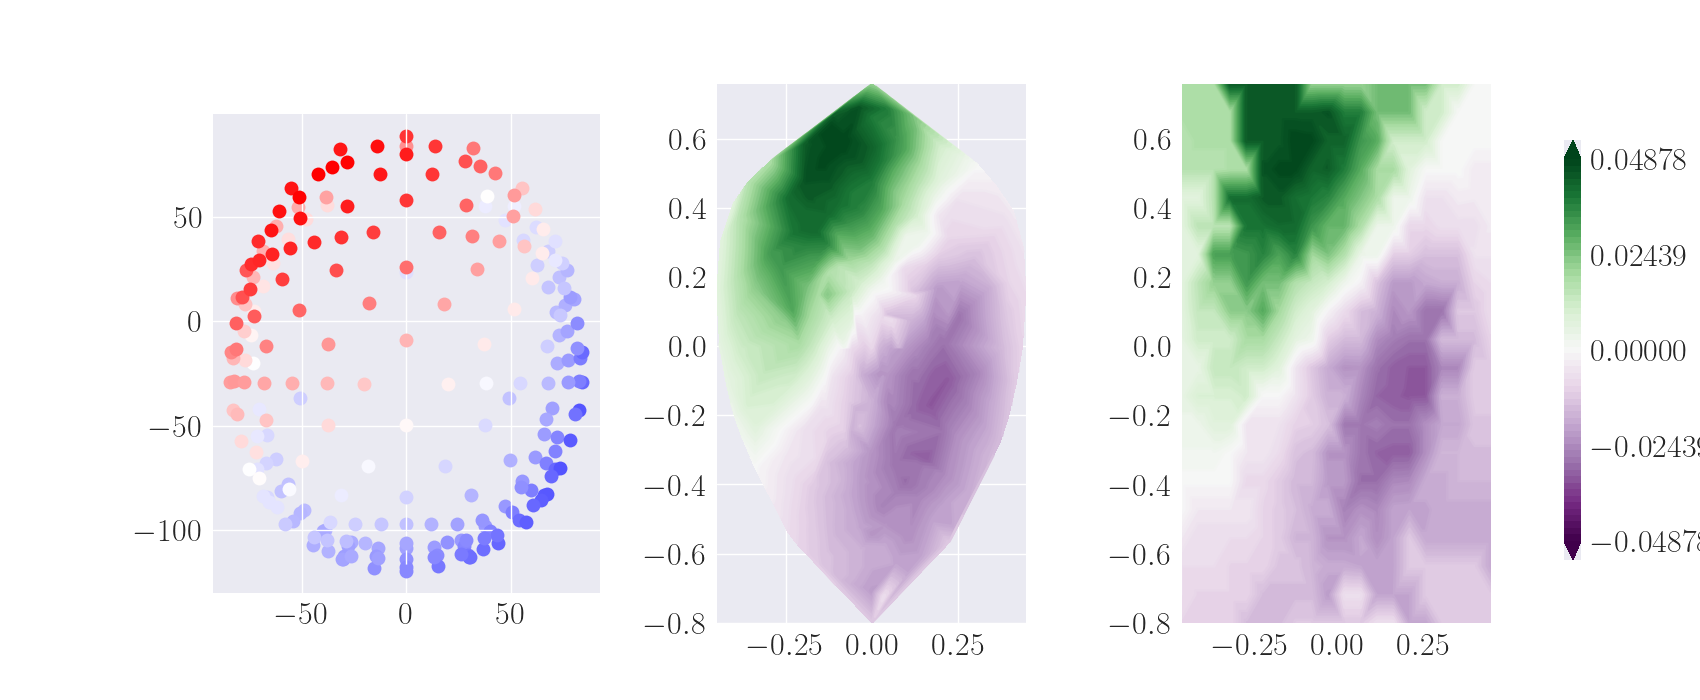
\includegraphics[width=\linewidth]{../Code/plots/finals/new_eeg_dipole_pos_6.png}

\caption{\newline
\textbf{Right}: EEG measure for 3 different samples measured in $\mu V$. \newline
\textbf{Middle and Left}: Illustration of the interpolation of the EEG data into two-dimensional matrix.}
\label{fig:eeg_dipole_pos_0}

\end{figure}

\begin{figure}[!htb]
    \centering
    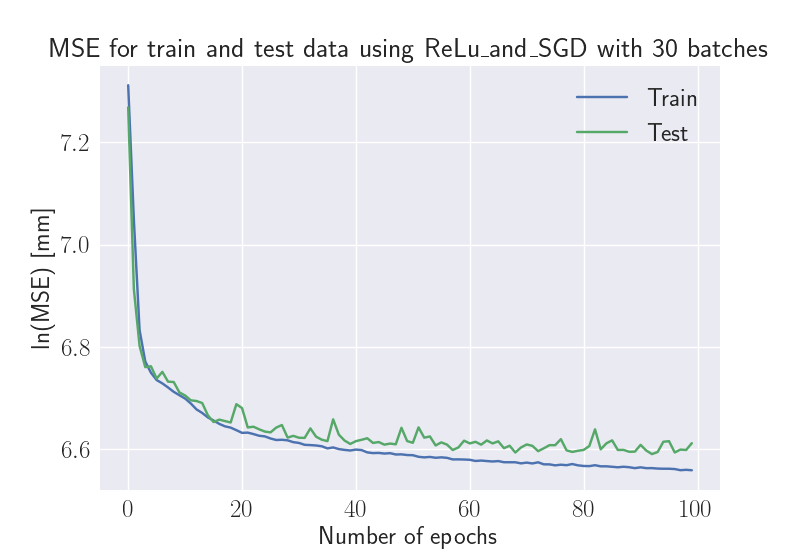
\includegraphics[width=\linewidth]{../Code/plots/finals/MSE_CNN_dipoles_2_interpolated_CNN_20x20_10000_ReLu_and_SGD_30_100.png}
    \caption{The validation accuracy for Convolutional Neural Network with 10 000 samples (20x20 matrix) with ReLU activation function. }
    \label{fig:single_dipole_accuracy_CNN_2d}
\end{figure}

% \begin{figure}[!htb]
%     \centering
%     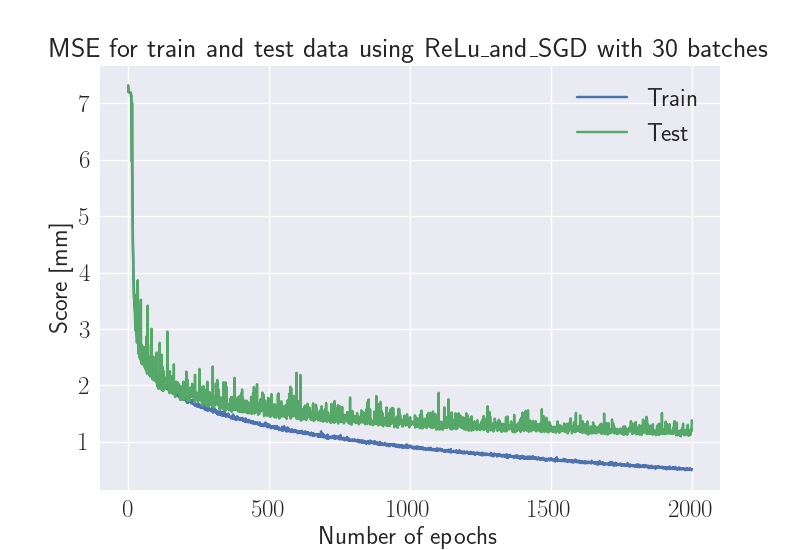
\includegraphics[width=\linewidth]{../Code/plots/CNN/MSE_interpolated_CNN_20x20_10000_ReLu_and_SGD_30_2000.png}
%     \caption{The validation accuracy for Convolutional Neural Network with 10 000 samples (20x20 interpolated matrix) with ReLU activation function. }
%     \label{fig:single_dipole_accuracy_CNN}
% \end{figure}


\section{Region of Active Correlated Current Dipoles}

Some results for the prediction of the size and location of current dipole populations.

\begin{figure}[!htb]
    \centering
    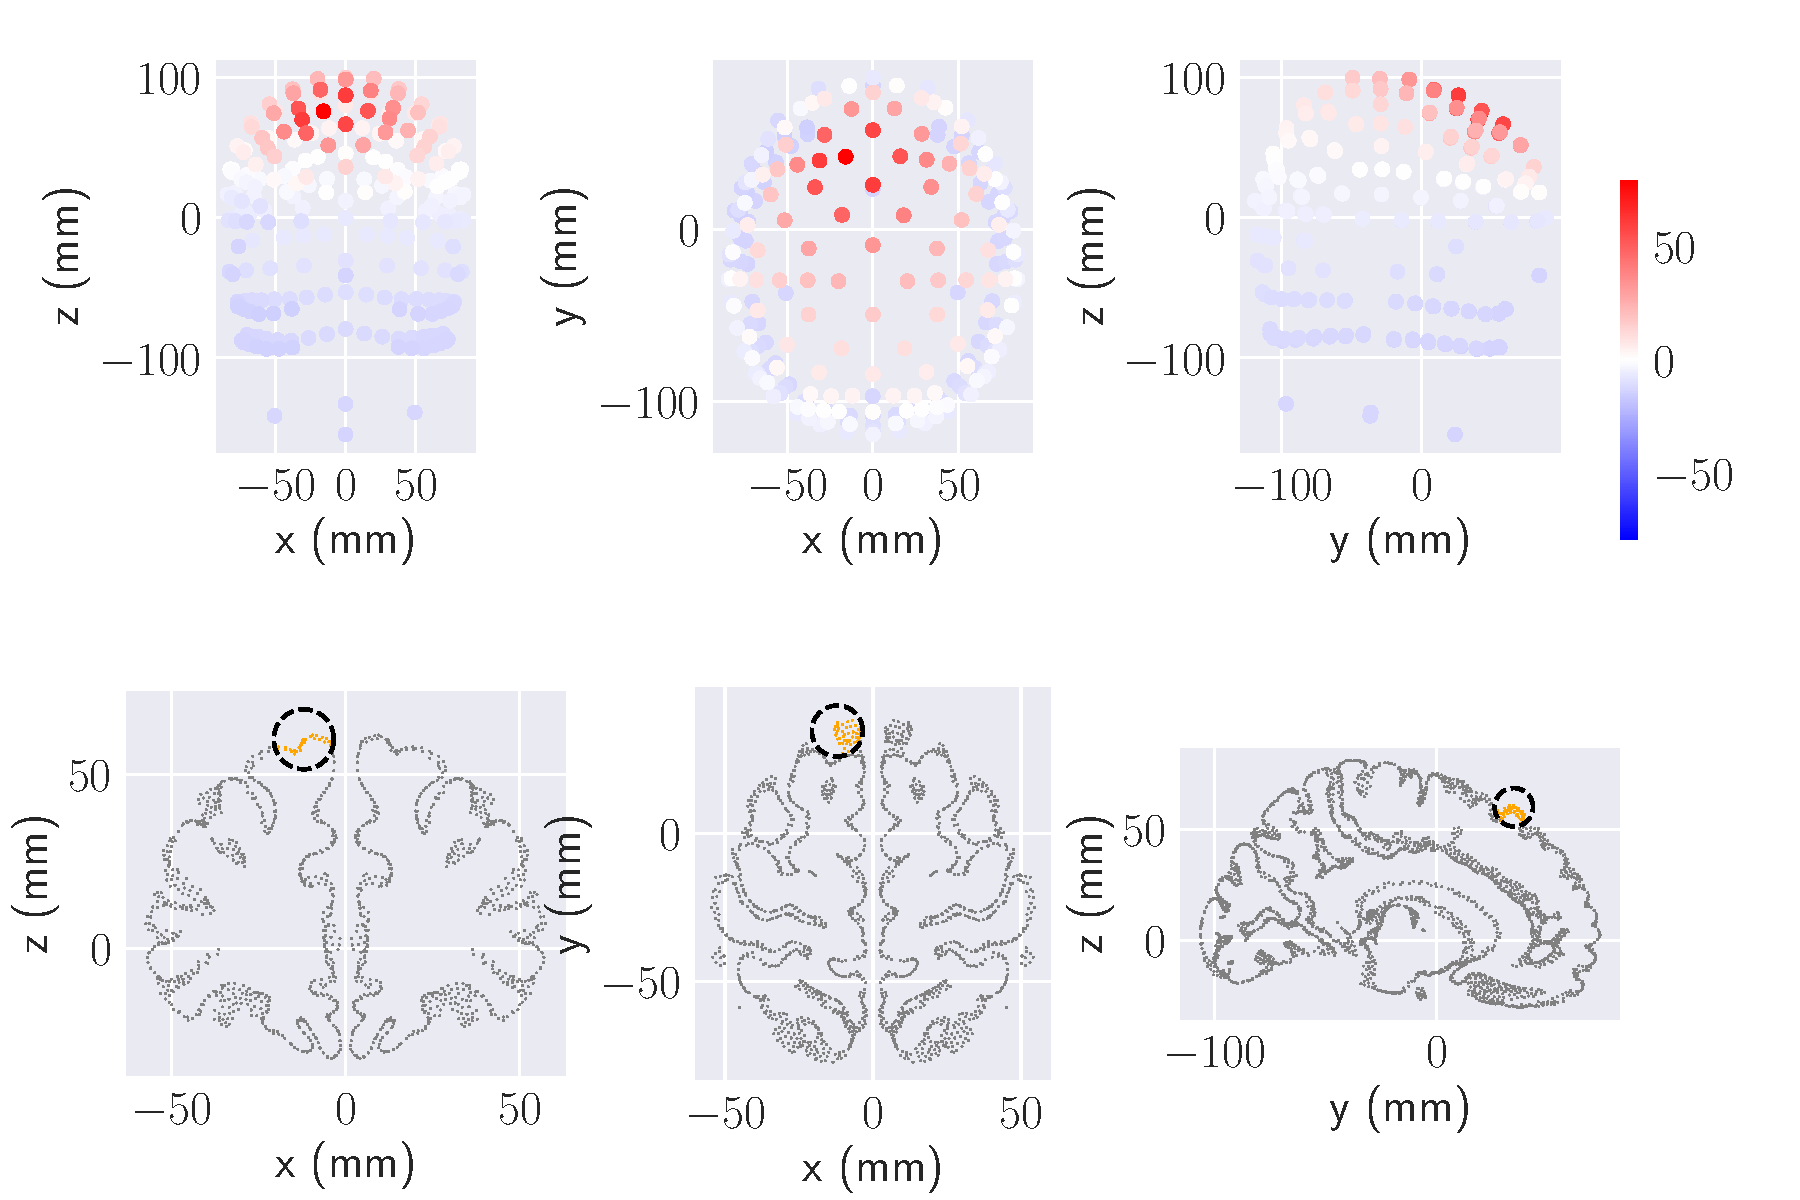
\includegraphics[width=\linewidth]{../Code/plots/finals/new_dipole_area_reduced_0.pdf}
    \caption{New text.}
    \label{fig:dipole_area}
\end{figure}

\begin{figure}[!htb]
    \centering
    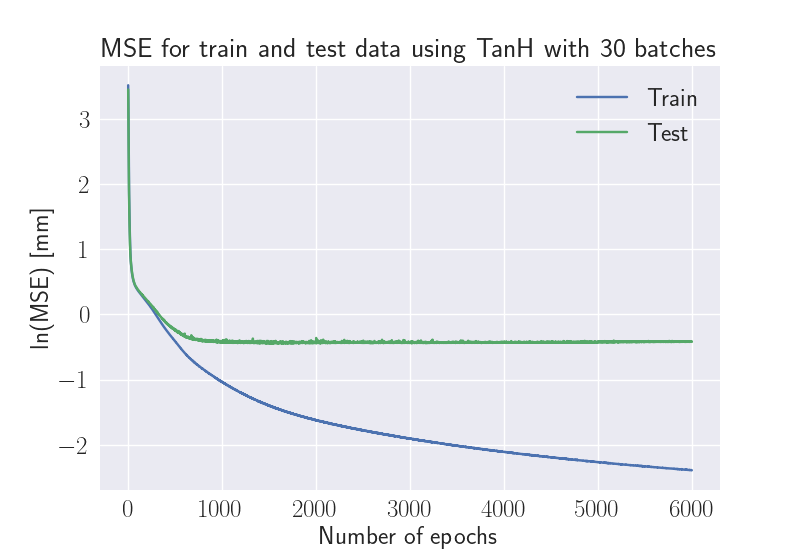
\includegraphics[width=\linewidth]{../Code/plots/finals/MSE_NN_1_10000_l1_l2_20mm_TanH_30_6000.png}
    \caption{New text.}
    \label{fig:dipole_area_result}
\end{figure}

\end{document}